\documentclass{article}
\usepackage[margin=1in]{geometry}
\usepackage{amsmath,amsfonts,amssymb}
\usepackage{listings}
\usepackage{color}
\usepackage{graphicx}
\usepackage{subfig}
\usepackage{blkarray}
\usepackage{multirow}
\usepackage{float}
\usepackage{caption}
\usepackage{subcaption}
\begin{document}
\begin{titlepage}
	\setlength{\parindent}{0pt}
	\large

\vspace*{-2cm}

\definecolor{dkgreen}{rgb}{0,0.6,0}
\definecolor{gray}{rgb}{0.5,0.5,0.5}
\definecolor{mauve}{rgb}{0.58,0,0.82}

\lstset{frame=tb,
  language=Python,
  aboveskip=3mm,
  belowskip=3mm,
  showstringspaces=false,
  columns=flexible,
  basicstyle={\small\ttfamily},
  numbers=none,
  numberstyle=\tiny\color{gray},
  keywordstyle=\color{blue},
  commentstyle=\color{dkgreen},
  stringstyle=\color{mauve},
  breaklines=true,
  breakatwhitespace=true,
  tabsize=3
}

University of Waterloo \par
CS 480 \par
\vspace{0.05cm}
r2knowle: 2023-11-28
\vspace{0.2cm}

{\huge Exercise \# 1 \par}
\hrule
\vspace{0.5cm}
\textbf{Q1a)} Below are some of the digits generated across the different epochs using my implementation of vae.py:
\begin{figure} [H]
\centering
\begin{tabular}{cccc}
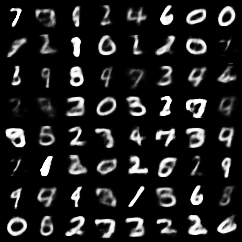
\includegraphics[width=0.3\textwidth]{sample_10.png} &
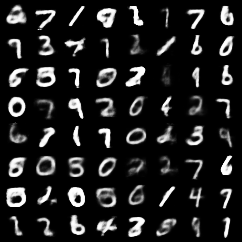
\includegraphics[width=0.3\textwidth]{sample_20.png} &
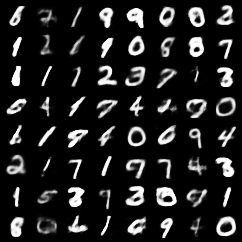
\includegraphics[width=0.3\textwidth]{sample_30.png} \\
\textbf{ Sample after Epoch 10 }  & \textbf{ Sample after Epoch 20 } & \textbf{ Sample after Epoch 30 }  \\[6pt]
\end{tabular}
\begin{tabular}{cccc}
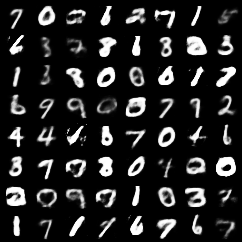
\includegraphics[width=0.3\textwidth]{sample_40.png} &
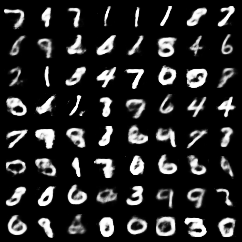
\includegraphics[width=0.3\textwidth]{sample_50.png} \\
\textbf{ Sample after Epoch 40 }  & \textbf{ Sample after Epoch 50 } 
\end{tabular}
\end{figure}
From this we can see that as the epochs increase, the quality of digits also seem to increase. We can seen that each digit becomes less epherial over time, and none are very clear from the start. We also get the following loss graph when generating these images using VAE:
\begin{center}
\begin{tabular}{cc}
\includegraphics[width=0.47\textwidth]{VANtest.png} & \includegraphics[width=0.47\textwidth]{VANtrain.png}
\end{tabular}
\end{center}
\newpage
\textbf{Q1b)} Below are some of the digits generated across the different epochs using my implementation of gan.py:
\begin{figure} [H]
\centering
\begin{tabular}{cccc}
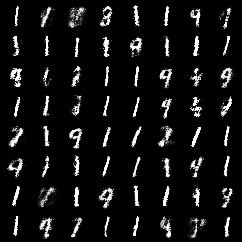
\includegraphics[width=0.3\textwidth]{sample_10_GAN.png} &
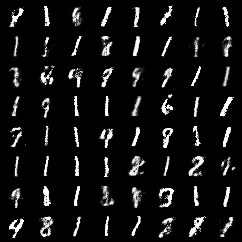
\includegraphics[width=0.3\textwidth]{sample_20_GAN.png} &
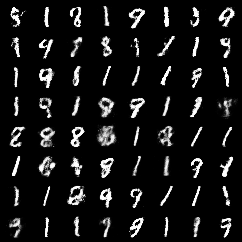
\includegraphics[width=0.3\textwidth]{sample_30_GAN.png} \\
\textbf{ Sample after Epoch 10 }  & \textbf{ Sample after Epoch 20 } & \textbf{ Sample after Epoch 30 }  \\[6pt]
\end{tabular}
\begin{tabular}{cccc}
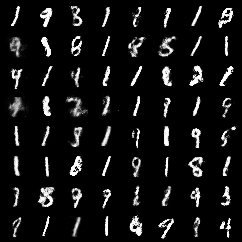
\includegraphics[width=0.3\textwidth]{sample_40_GAN.png} &
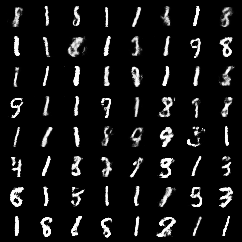
\includegraphics[width=0.3\textwidth]{sample_50_GAN.png} \\
\textbf{ Sample after Epoch 40 }  & \textbf{ Sample after Epoch 50 } 
\end{tabular}
\end{figure}
From this we can see that as the epochs increase, the quality of digits also seem to increase. We also see that 1 is prioritized most likely becomes it is easy to generate and is hard for the discriminator to detect. We also get the following loss graph when generating these images using GAN:
\begin{center}
\begin{tabular}{cc}
\includegraphics[width=0.47\textwidth]{gantest.png} & 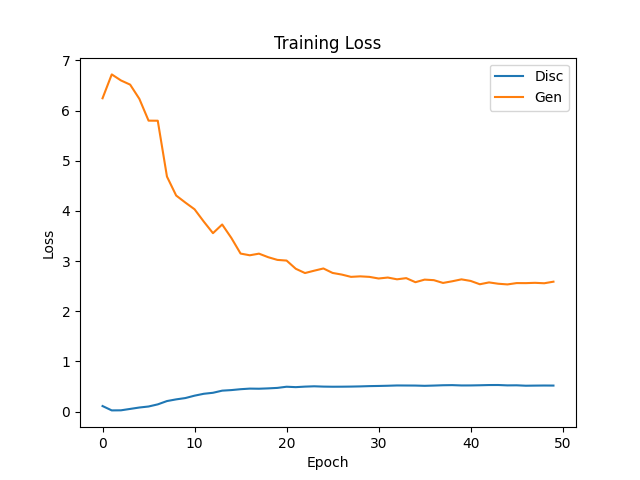
\includegraphics[width=0.47\textwidth]{ganloss.png}
\end{tabular}
\end{center}
\newpage
\textbf{Q1c)} One of the most important observations is that VAE tends to uniformly create digits where as GAN tends to create specific digits. This is due to the fact that specific digits (like 1) are harder to detect then other digits, as they are more simple and easier to generate, this should sway the generator to make more of them to minimize loss as we dont care about which digit is created. For the GAN we can see that one is generated quite a bit, but thats also due to the fact that 1 is similar to a stem that is shared by 1,4,7,9.
\end{titlepage}
\end{document}